\documentclass[11pt,a4paper]{article}
\usepackage[utf8]{inputenc}
\usepackage[T1]{fontenc}
\usepackage[english]{babel}
\usepackage{lmodern}
\usepackage{microtype}
\usepackage{geometry}
\usepackage{hyperref}
\usepackage{graphicx}
\geometry{margin=2.7cm}

\title{From Complex Structures to Fiction:\\A Spatial Approach to European Storytelling}
\author{Francesco Sisini}
\date{}

\begin{document}
\maketitle

\begin{abstract}
Contemporary Europe is traversed by scientific, technological, energy, economic, and institutional structures distributed across different territories and difficult to observe in their entirety from any single local scale. This work proposes taking such structures as the starting point for constructing narratives set within the European space. The method uses a shared Geographic Information System (GIS) in which existing structures, or sufficiently plausible future developments of them, are reconstructed through their components, geographic distribution, and relations. The process can be summarized as real structure → GIS reconstruction → observation → narrative possibility → story. The map is therefore not constructed to represent an already existing story: observation of the structure precedes the story and contributes to its generation. As a first case study, the paper presents the geographic reconstruction of the nuclear fuel cycle and the subsequent development of the story Quantum Reactor. Finally, the GIS constitutes an open and extensible environment in which structures and narratives can accumulate independently, allowing different stories to share and traverse the same representation of European space.
\end{abstract}

\noindent\textbf{Keywords:} narrative structures; complex systems; spatial
narrative; electronic literature; European storytelling; literary cartography;
practice-based research.

\section{Introduction: From Systems in Fiction to Systems as Generators of Fiction}

\subsection{From Scientific Knowledge to Complex Structures}

The progressive formalization of scientific knowledge and its translation into technology have profoundly characterized the nineteenth, twentieth, and twenty-first centuries. From the Eiffel Tower to large hydroelectric power plants, human ingenuity has shaped the territory through works that demonstrate the ability to translate knowledge increasingly connected with scientific research into technology.

Naturally, the ability to construct complex works predates the scientific revolution by many centuries. Temples, aqueducts, and cathedrals testify to extremely sophisticated geometric, technical, and empirical knowledge. What progressively changes is the relationship between knowledge and design. Knowledge based on materials, proportions, and previously tested techniques is joined by physical and mathematical models capable of predicting the behavior of structures even under conditions not previously experienced \cite{quarteroni2009,eckert2022}. Scientific knowledge thus becomes a generative tool for designing what does not yet exist, in addition to supporting the understanding of existing systems.

This transformation has also changed the organization of society and its systems of production and distribution. A truck supplying flour to a city far from agricultural areas is the visible point of a much larger structure: cultivated fields, agricultural machinery, processing plants, silos, transport infrastructure, and distribution networks. Similarly, an emergency procedure in a peripheral hospital depends on systems for the production and distribution of medicines, electrical grids, drinking water, transport, and communications. A local action may therefore depend on the operation of a complex and geographically distributed structure; in the case of agri-food supply chains, the literature explicitly describes chains composed of different actors, forms of coordination, and governance relations \cite{carbone2017}.

\subsection{The Loss of Self-Similarity}
A useful image for describing this transformation is provided by the mathematical concept of self-similarity. In the Sierpiński triangle, the form observed at a given scale reproduces the structure visible at different scales \cite{palagallo2004}. With some latitude, and without assigning a rigorous mathematical meaning to the analogy, something similar can be recognized in certain forms of productive organization in the past: managing a small portion of land could reproduce many of the activities involved in the agricultural management of an entire estate.

Today this symmetry appears much less evident. In the operations of a small farmer, it is difficult to recognize the structure of the current global system of cereal production and distribution, which is composed of different and specialized elements. Contemporary society contains macrostructures that do not reappear, in reduced form, at intermediate or local scales. The individual element is not necessarily a scaled representation of the overall system: understanding the system therefore requires reconstructing its components, functions, relations, flows, and dependencies.

Without entering the much broader field of the relationship between literature and the evolution of society, we can ask how narrative might accompany this transformation as well. If the overall system is not self-similar to its individual components, we cannot assume that its representation will necessarily emerge from the accumulation of local stories. Telling the story of a farmer, a doctor, a technician, or an employee may accurately describe their experience without making visible the macrostructure of which they constitute a node.
\subsection{Complex Structures as Starting Points for Fiction}
From this consideration arises the project, presented here for the first time in formal terms, of a method of narrative construction that takes as its direct starting point some of the large complex structures through which contemporary society operates. The structure is studied as a whole, identifying its components, geographic distribution, functions, relations, flows, and dependencies; only afterwards are narrative possibilities sought within it.

The project considers in particular structures operating at a European scale, whether already existing or plausibly future. A first example is the system required to manage the nuclear fuel cycle, from the production and transformation of raw materials to infrastructures for research, use, and control. From this reconstruction, the story \emph{Quantum Reactor} was developed and is used below as the first case study. The same approach can be applied to economic and financial systems or to emerging European infrastructures in the digital and artificial-intelligence domains.

The hypothesis explored here is therefore that these macrostructures can serve as starting points for the creative process. They are studied before the story exists, allowing narrative possibilities to emerge from their components and relations.


\section{Literature and Complex Systems}

Before describing the project proposed here, it is useful to consider some apparently analogous experiences in recent literature. A particularly emblematic case is that of the American writer Michael Crichton, whose work frequently transformed scientific, technological, and economic knowledge into central elements of narrative construction. This reading is supported by criticism that places Crichton's interest in the social consequences of science and technology within a broader perspective than the conventional techno-thriller classification \cite{stengler2015}.

In \emph{Jurassic Park}, for example, the possibility of reconstructing extinct organisms through DNA is accompanied by the problem of predicting and controlling the evolution of a complex system. Chaos theory, explicitly invoked through the character of Ian Malcolm, participates directly in the narrative mechanism. It is also significant that Crichton himself described a long evolution of the narrative idea: from a 1983 screenplay about cloning a pterodactyl from fossil DNA to the later choice of a theme park as the structure of the story \cite{crichtonJP}. A similar procedure, applied to different domains, can be recognized in \emph{Rising Sun}, where a particular story makes it possible to observe economic, industrial, and technological relations between the United States and Japan, and in \emph{Airframe}, where the investigation of an accident provides a path through the technical and organizational system of the aviation industry.

In these works, the narrative problem does not therefore necessarily arise from the psychological observation of the characters alone. Scientific concepts, technological systems, and economic structures themselves become narrative material, while the characters allow the reader to experience their consequences. From this perspective, Crichton represents a particularly interesting precedent for the approach proposed here: theoretical knowledge and complex systems can themselves become generative elements of literature alongside feelings, relationships, and individual situations.

A further movement toward the direction explored here can be recognized in \emph{Congo}. In this novel it is more difficult to identify a single principle from which the narrative develops. Instead, elements belonging to different domains converge: primatology, geographic exploration, technology, logistics, mineral resources, economic interests, and archaeology. It is the relationship among these elements, made possible by the expedition around which the novel develops, that progressively constructs the narrative space.

The discontinuity with the approach proposed in this work becomes less clear here. The further step we intend to explore consists in deliberately placing at the origin of the process a structure that exists independently of the story. Its components and relations are reconstructed before the narrative is defined. The initial question therefore concerns the stories that may emerge from the observation of a real structure. This shift concerns the starting point of narrative construction and imposes no constraints on its subsequent development: a story generated through the observation of a macrostructure can naturally develop characters, feelings, relationships, and conflicts using the same tools as any other form of narrative.


\section{Proposed Method: Complex Structures as Narrative Generators}

\subsection{A Shared Geographic Model}

\begin{figure}[htbp]
    \centering
    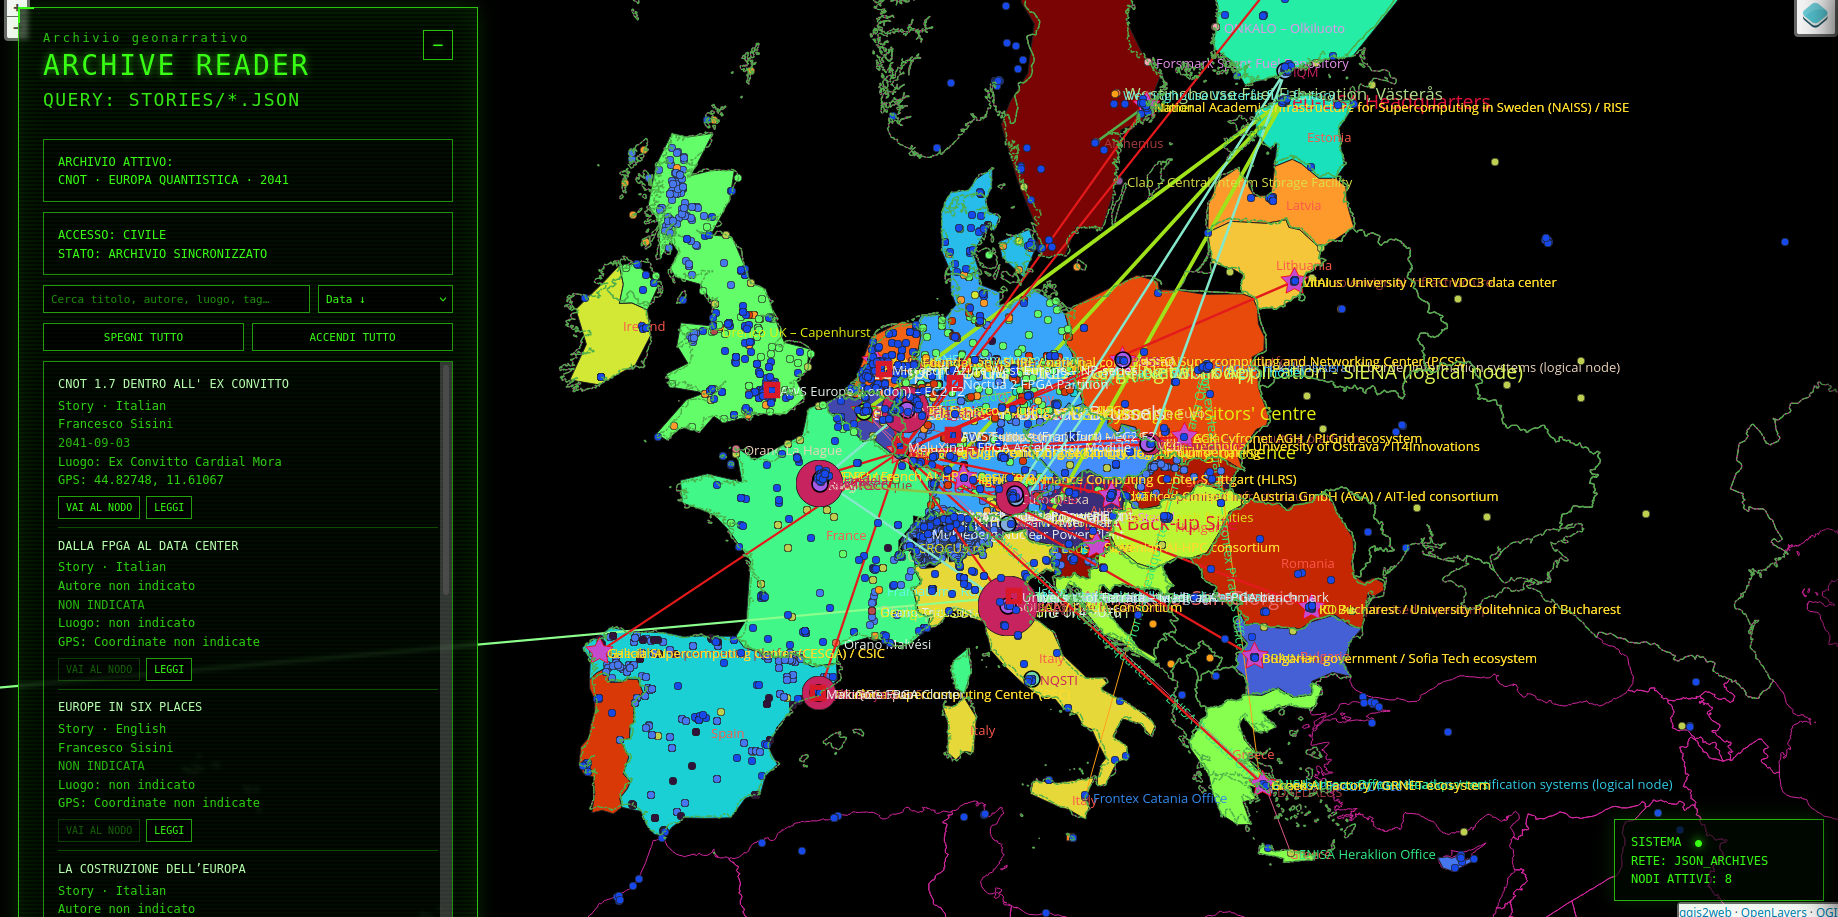
\includegraphics[width=\linewidth]{pictures/gis1.png}
    \caption{The CNOT Archive Reader and the shared European GIS environment.}
    \label{fig:gis-archive-reader}
\end{figure}


The proposed method uses a shared Geographic Information System (GIS) to represent existing or possible European structures that are geographically distributed, for example political, scientific, energy, economic, and technological structures. These use the concept of layers to describe locatable components and, where possible, the relations connecting them.

The GIS represents a portion of the world from which stories may emerge. This use belongs to a broader context of studies on literary cartography and digital spatial narrative, in which maps and interactive geographic environments can take an active role in the analysis or construction of narrative \cite{reuschel2011,cerri2025,mai2021}. Historical, documentary, or literary narratives can subsequently be associated within the same environment, while keeping the structural and narrative levels distinct.

\subsection{From Structures to Narratives}

The process can be summarized as:
\[
\mathrm{real\ structure}
\rightarrow
\mathrm{GIS\ reconstruction}
\rightarrow
\mathrm{observation}
\rightarrow
\mathrm{narrative\ possibility}
\rightarrow
\mathrm{story}.
\]

The inversion with respect to an illustrative use of cartography is essential. A structure is first constructed through its components, geographic distribution, functions, and relations. The author then observes this structure in search of the narrative possibilities it contains. The GIS therefore constitutes a generative, not prescriptive, tool: characters, conflicts, and the development of the story remain free.

\subsection{An Open and Extensible European Narrative Space}

\begin{figure}[htbp]
    \centering
    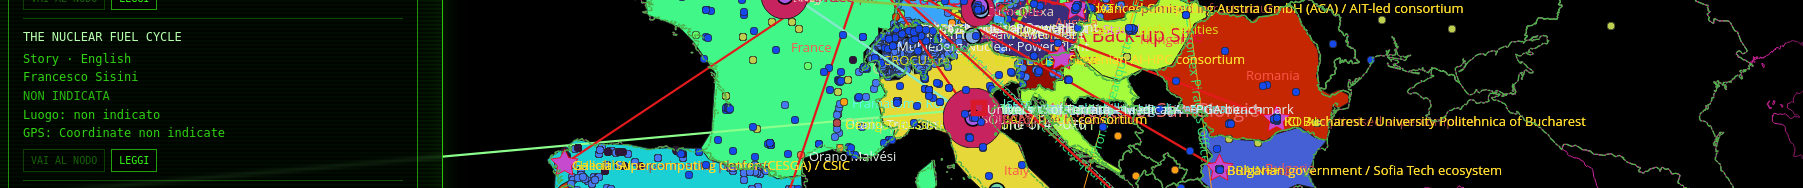
\includegraphics[width=\linewidth]{pictures/gis2.png}
    \caption{A narrative entry associated with the Nuclear Fuel Cycle in the GIS archive.}
    \label{fig:gis-nuclear-entry}
\end{figure}


The model is cumulative: structures and information added for one narrative remain available for subsequent ones, while multiple stories can traverse the same geographic elements.

A first experimental implementation is being developed in the open-source CNOT Franchise project,\footnote{\url{https://github.com/francescosisini/Cnot-Franchise}} which includes an interactive GIS\footnote{\url{https://francescosisini.github.io/Cnot-Franchise/gis/reader.html}} in which structural layers and narratives coexist within the same environment.

The GIS therefore constitutes a persistent and extensible representation of European space: new information can suggest new narratives, and new narratives can indicate parts of the structure that deserve further investigation.


\section{Case Study: From the Nuclear Fuel Cycle to \emph{Quantum Reactor}}

\subsection{Reconstructing the Nuclear Fuel Cycle}

\begin{figure}[htbp]
    \centering
    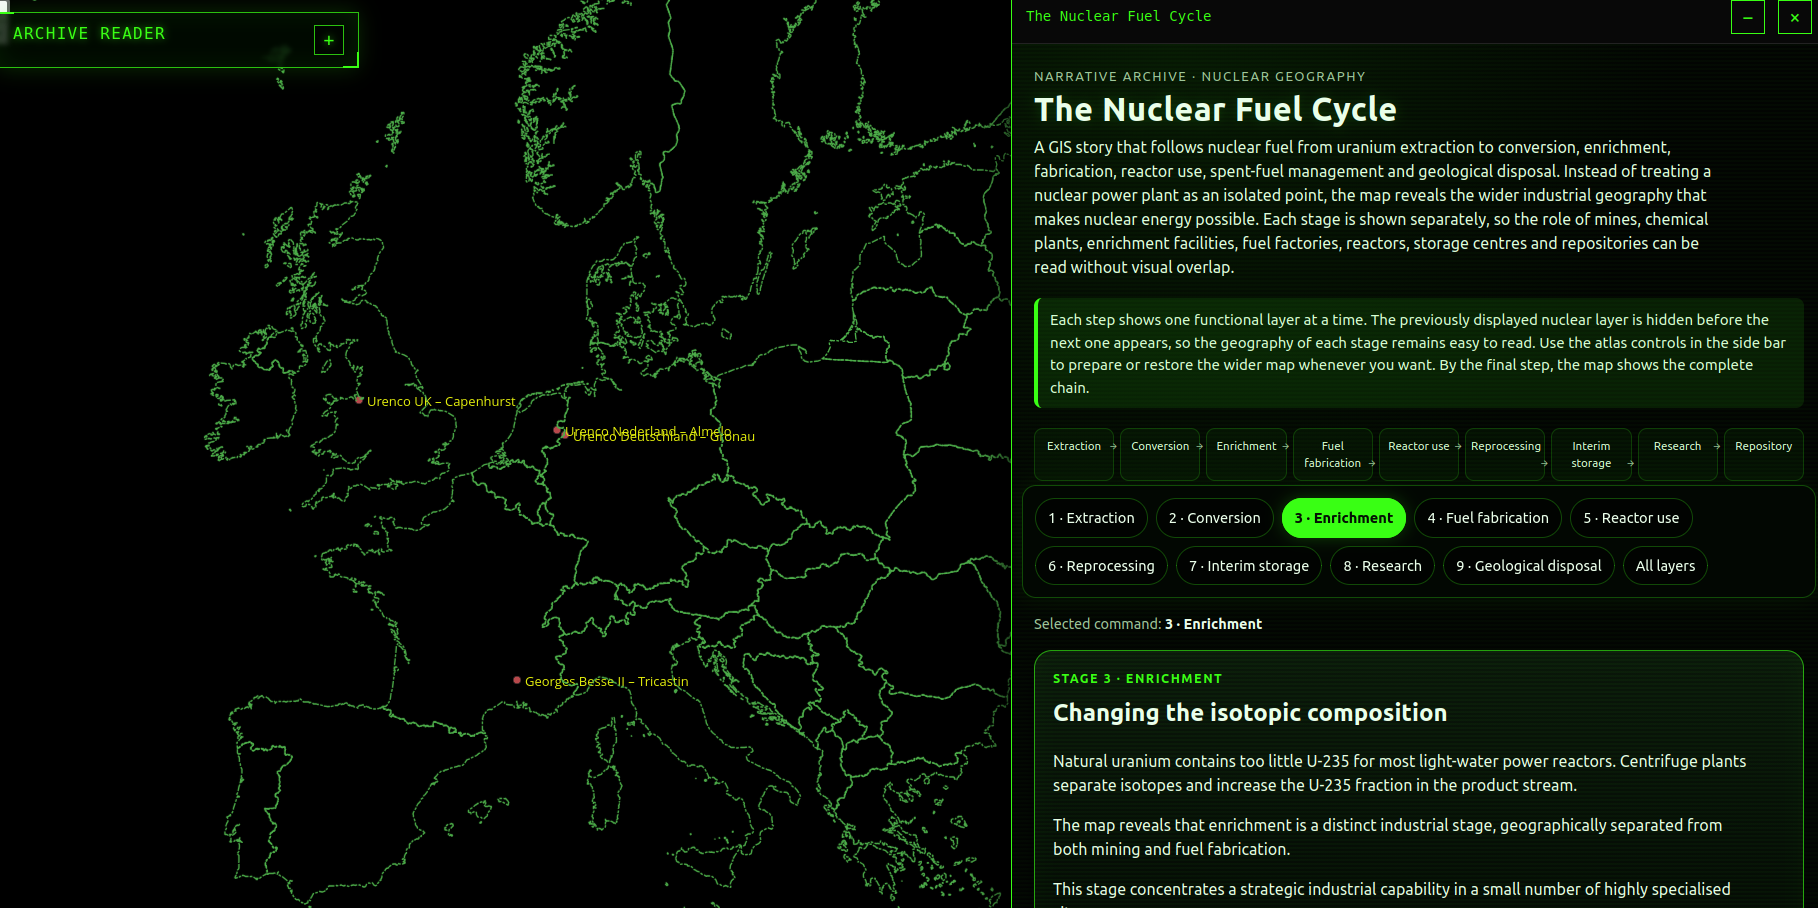
\includegraphics[width=\linewidth]{pictures/gis3.png}
    \caption{Interactive representation of the Nuclear Fuel Cycle, showing the enrichment stage.}
    \label{fig:gis-fuel-cycle}
\end{figure}


The nuclear fuel cycle was selected as the first experimental case. Before the story was defined, the system was reconstructed in the GIS by identifying the main stages leading from raw material to fuel usable in a reactor and to the subsequent production of energy. Sites related, among others, to uranium extraction, conversion, enrichment, fuel fabrication, energy production, and nuclear research were therefore considered. The sequence of the main stages of the cycle is consistent with the description adopted by the International Atomic Energy Agency \cite{iaeaFuelCycle}.

These elements, normally described separately, were represented within the same geographic space through dedicated layers. The result at this stage is a representation of the distributed structure that makes the nuclear fuel cycle possible, prior to the development of a narrative.

\subsection{From Geographic Structure to Narrative}

Observation of the structure immediately revealed a feature that could be used narratively: the different stages of the cycle correspond to geographically separate locations connected by flows of materials, knowledge, technologies, and procedures. The structure itself therefore suggests the possibility of a path through its nodes.

From this observation emerged the idea of a character who, for reasons related to his work, progressively moves through different components of the system. The narrative problem then became that of identifying a plausible reason for this movement and an element capable of connecting the different visits. From this process, the central elements of the story progressively emerged: an anomalous scientific investigation, an apparently impossible paper, the need to inspect different sites in the nuclear cycle, and a series of clues observable along the route.

The process actually followed can therefore be schematized as:

\[
\mathrm{Nuclear\ Fuel\ Cycle}
\rightarrow
\mathrm{GIS}
\rightarrow
\mathrm{geographic\ observation}
\rightarrow
\mathrm{path\ through\ nodes}
\rightarrow
\mathrm{narrative\ hypothesis}.
\]

In this case, therefore, geographic distribution was not added to the story afterwards: it contributed directly to its generation.

\subsection{\emph{Quantum Reactor}: The Resulting Story}

\begin{figure}[htbp]
    \centering
    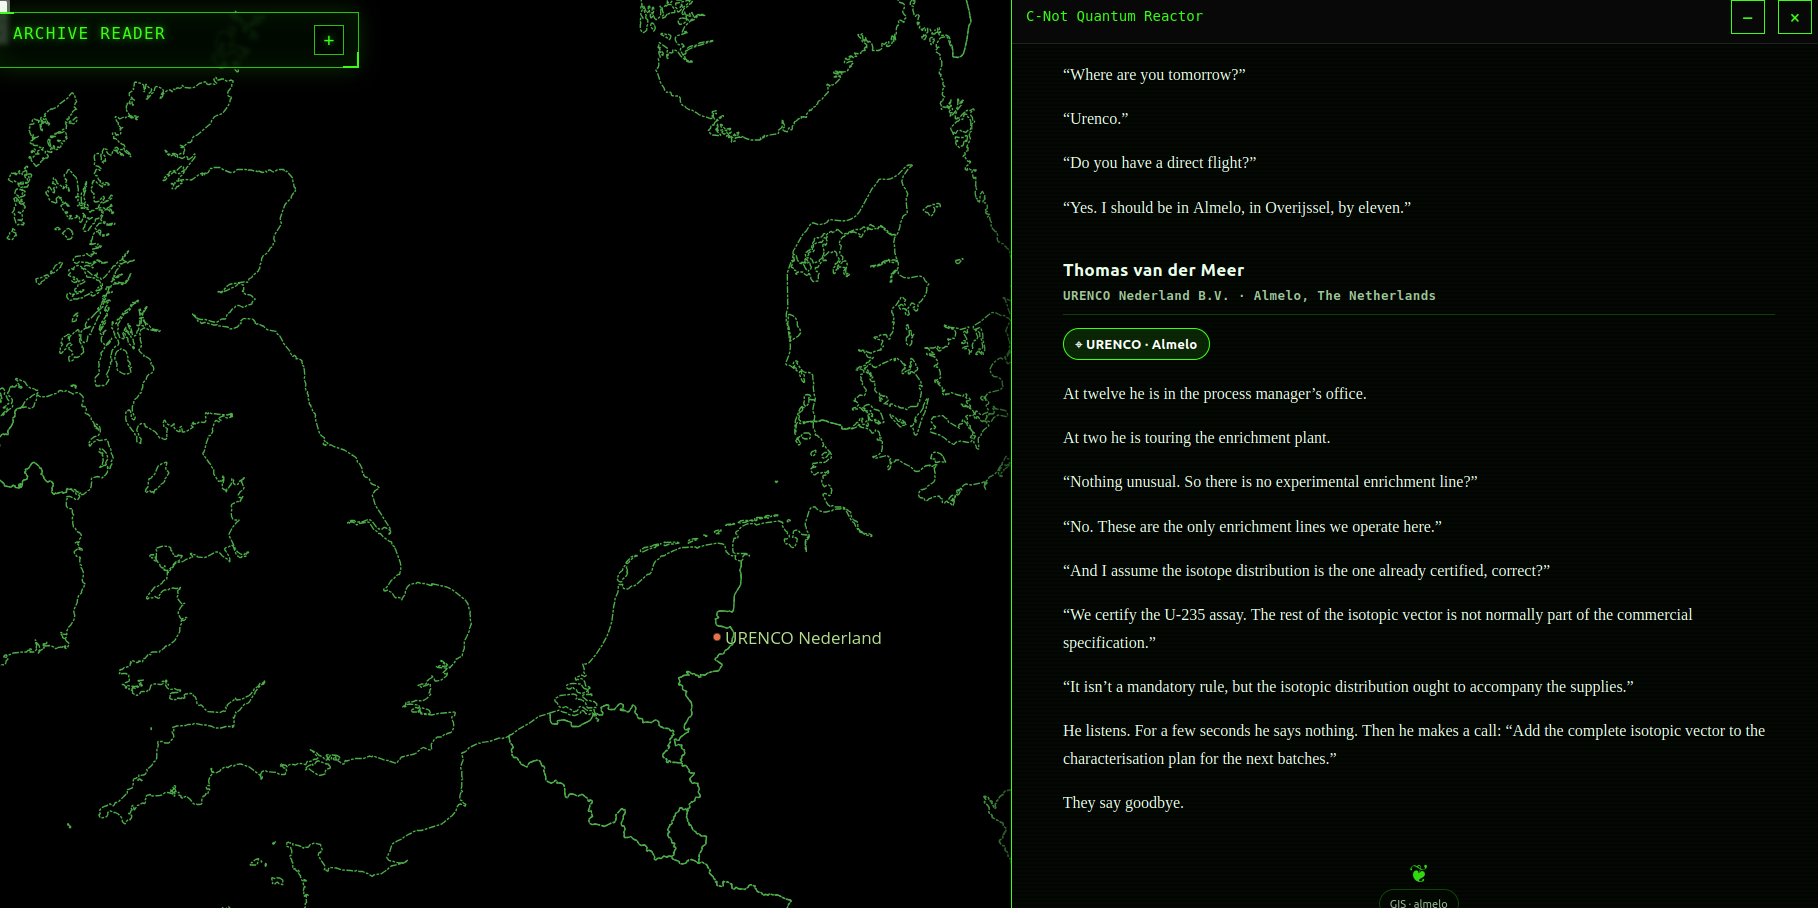
\includegraphics[width=\linewidth]{pictures/gis4.png}
    \caption{\emph{Quantum Reactor} displayed together with the geographic node associated with the narrative.}
    \label{fig:gis-quantum-reactor}
\end{figure}


The result of this process is the story \emph{Quantum Reactor}. The narrative follows a path through different nodes of the nuclear cycle, using the previously reconstructed structure as the geographic and technological framework of the story. Fictional elements are therefore superimposed on a structure that had been studied independently of its subsequent narrative use.

Once completed, the story is in turn inserted into the same GIS and can interact with the structural layers from which it was generated. The process therefore takes on a circular form:

\[
\mathrm{structure}
\rightarrow
\mathrm{GIS}
\rightarrow
\mathrm{narrative}
\rightarrow
\mathrm{GIS}.
\]

\emph{Quantum Reactor} therefore constitutes a first experiment with the proposed method: the structure precedes the narrative, contributes to its generation, and remains available, independently of the individual story, as a basis for further narrative explorations.





\section{Conclusions}

This work has proposed a method of narrative construction in which complex structures, whether real or plausibly future, are reconstructed and observed through a GIS before the story is defined. The central hypothesis is that the geographic representation of infrastructures, institutions, flows, and relations can make observable features of contemporary society that are difficult to recognize from the local scale alone and, at the same time, suggest new narrative possibilities.

The GIS therefore assumes a dual function. On the one hand, it constitutes a research and construction tool for the author; on the other, it can become an open environment in which different structures and narratives are progressively collected and related to one another. In this sense, we can provisionally define as \emph{GIS-based narratives} historical, documentary, or fictional stories that use this shared geographic space and the structures represented within it.

The GIS-based nature of the construction does not, however, imply that the GIS must constitute the final form of the work. A narrative generated through this method can be read interactively together with the geographic structure from which it emerged. It can also be published independently in traditional literary forms, including the book. The GIS therefore belongs to the generative process and constitutes a possible extension of the reading experience without constraining the final medium.

The case of \emph{Quantum Reactor} represents a first experiment with this process: the geographic reconstruction of the nuclear fuel cycle preceded the definition of the story and contributed to the construction of its narrative path. The same story can subsequently be published as an autonomous work while retaining its connection with the geographic environment that contributed to its generation.

The project remains intentionally open. New European structures can be added to the GIS and made available for new narratives; similarly, different authors can use, extend, or traverse existing structures in different ways. The objective is therefore to experiment with a shared space in which geographic knowledge, observation of complex structures, and narrative construction can mutually reinforce one another, without defining a new closed literary genre.



\begin{thebibliography}{99}

\bibitem{quarteroni2009}
A. Quarteroni,
``Mathematical Models in Science and Engineering,''
\emph{Notices of the American Mathematical Society},
vol.~56, no.~1, pp.~10--19, 2009.

\bibitem{eckert2022}
C. Eckert and R. Hillerbrand,
``Models in Engineering Design as Decision-Making Aids,''
\emph{Engineering Studies},
vol.~14, no.~2, pp.~134--157, 2022.
doi: 10.1080/19378629.2022.2129061.

\bibitem{carbone2017}
A. Carbone,
``Food supply chains: coordination governance and other shaping forces,''
\emph{Agricultural and Food Economics},
vol.~5, article 3, 2017.
doi: 10.1186/s40100-017-0071-3.

\bibitem{palagallo2004}
J. A. Palagallo and M. Palmer,
``Analysis of an Irregular Sierpinski Triangle,''
\emph{Fractals},
vol.~12, no.~1, pp.~137--144, 2004.
doi: 10.1142/S0218348X04002239.

\bibitem{reuschel2011}
A.-K. Reuschel and L. Hurni,
``Mapping Literature: Visualisation of Spatial Uncertainty in Fiction,''
\emph{The Cartographic Journal},
vol.~48, no.~4, pp.~293--308, 2011.
doi: 10.1179/1743277411Y.0000000023.

\bibitem{cerri2025}
M. Cerri,
``From Chronology to Cartography: Spatial Configurations in Three Works of Electronic Literature,''
\emph{Interface -- Journal of European Languages and Literatures},
no.~26, pp.~101--124, 2025.
doi: 10.6667/interface.26.2025.251.

\bibitem{mai2021}
G. Mai, W. Huang, L. Cai, R. Zhu, and N. Lao,
``Narrative Cartography with Knowledge Graphs,''
arXiv:2112.00970, 2021.

\bibitem{stengler2015}
E. Stengler,
``Beyond the Techno-thriller: Michael Crichton and Societal Issues in Science and Technology,''
\emph{Fafnir -- Nordic Journal of Science Fiction and Fantasy Research},
vol.~2, no.~3, pp.~23--30, 2015.

\bibitem{crichtonJP}
M. Crichton,
``Jurassic Park -- In His Own Words,''
Michael Crichton official website.
\url{https://michaelcrichton.com/works/jurassic-park/}
Accessed August 9, 2026.

\bibitem{iaeaFuelCycle}
International Atomic Energy Agency,
\emph{The Nuclear Fuel Cycle}.
Vienna: IAEA.
\url{https://www.iaea.org/sites/default/files/19/02/the-nuclear-fuel-cycle.pdf}
Accessed August 9, 2026.

\end{thebibliography}

\end{document}
